% s1_s2_tikz_diagrams.tex
\documentclass{standalone}
\usepackage{tikz}
\usepackage{amsmath, amssymb}
\newcommand{\R}{\mathbb{R}}
\begin{document}
	
	% Step 1: The circle S^1 in the plane
	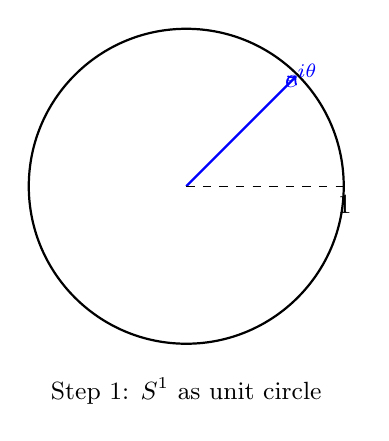
\begin{tikzpicture}[scale=2]
		\draw[thick] (0,0) circle(1);
		\coordinate (P) at (0.7,0.7);
		\draw[->,thick,blue] (0,0) -- (P) node[pos=0.8, above right] {$e^{i\theta}$};
		\draw[dashed] (0,0) -- (1,0) node[pos=0.9, below right] {1};
		\node at (0,-1.3) {\small Step 1: $S^1$ as unit circle};
	\end{tikzpicture}
	
	% Step 2: Planar rotation by theta
	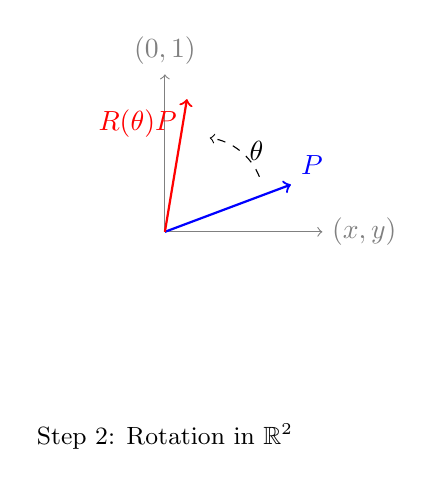
\begin{tikzpicture}[scale=2]
		\draw[->,gray] (0,0) -- (1,0) node[right] {$(x,y)$};
		\draw[->,gray] (0,0) -- (0,1) node[above] {$(0,1)$};
		\coordinate (P0) at (0.8,0.3);
		\coordinate (P1) at ({0.8*cos(60)-0.3*sin(60)},{0.8*sin(60)+0.3*cos(60)});
		\draw[->,thick,blue] (0,0) -- (P0) node[above right] {$P$};
		\draw[->,thick,red]  (0,0) -- (P1) node[below left] {$R(\theta)P$};
		\draw[->,dashed] (0.6,0.35) arc[start angle=22,end angle=82,radius=0.4] 
		node[midway, right] {$\theta$};
		\node at (0,-1.3) {\small Step 2: Rotation in $\R^2$};
	\end{tikzpicture}
	
	% Step 3: Embedding into R^3 (fix z-axis)
	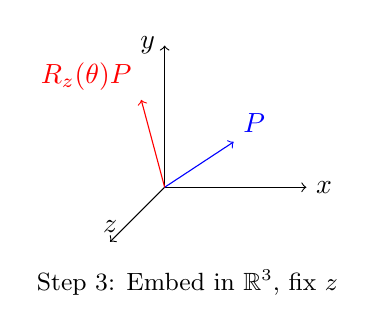
\begin{tikzpicture}[scale=1.5]
		% axes
		\draw[->] (0,0,0) -- (1.2,0,0) node[right] {$x$};
		\draw[->] (0,0,0) -- (0,1.2,0) node[left] {$y$};
		\draw[->] (0,0,0) -- (0,0,1.2) node[above] {$z$};
		% point and rotation
		\coordinate (P3) at (0.7,0.5,0.3);
		\coordinate (P3r) at ({0.7*cos(60)-0.5*sin(60)},{0.7*sin(60)+0.5*cos(60)},0.3);
		\draw[->,blue] (0,0,0) -- (P3) node[above right] {$P$};
		\draw[->,red]  (0,0,0) -- (P3r) node[above left] {$R_z(\theta)P$};
		\node at (0,-1,-0.5) {\small Step 3: Embed in $\R^3$, fix $z$};
	\end{tikzpicture}
	
	% Step 4: Action on the sphere S^2
	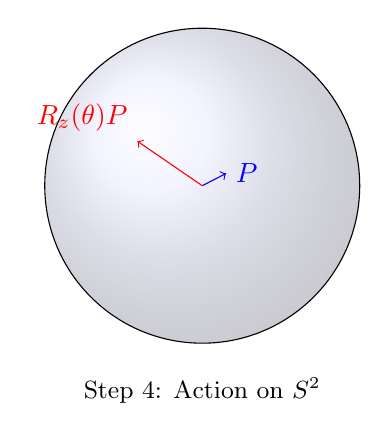
\begin{tikzpicture}[scale=2]
		% draw circle for great circle
		\shade[ball color=white!80!blue,opacity=0.3] (0,0) circle (1);
		\draw (0,0) circle (1);
		% points
		\coordinate (P4) at ({0.6*cos(40)},{0.6*sin(40)});
		\coordinate (P4s) at ({0.6*cos(40)},{0.6*sin(40)}, {sqrt(1-0.6^2)});
		\coordinate (P4r) at ({(0.6*cos(40))*cos(60)-(0.6*sin(40))*sin(60)},{(0.6*cos(40))*sin(60)+(0.6*sin(40))*cos(60)},{sqrt(1-0.6^2)});
		\draw[->,blue] (0,0) -- (P4s) node[right] {$P$};
		\draw[->,red]  (0,0) -- (P4r) node[above left] {$R_z(\theta)P$};
		\node at (0,-1.3) {\small Step 4: Action on $S^2$};
	\end{tikzpicture}
	
	% Step 5: Group axioms visually (composition)
	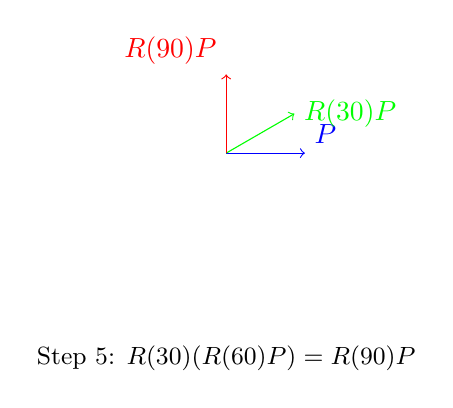
\begin{tikzpicture}[scale=2]
		\coordinate (P0) at (0.5,0);
		\coordinate (P1) at ({0.5*cos(30)-0*sin(30)},{0.5*sin(30)+0*cos(30)});
		\coordinate (P2) at ({0.5*cos(30+60)},{0.5*sin(30+60)});
		\draw[->,blue]  (0,0) -- (P0) node[above right] {$P$};
		\draw[->,green] (0,0) -- (P1) node[right] {$R(30°)P$};
		\draw[->,red]   (0,0) -- (P2) node[above left] {$R(90°)P$};
		\node at (0,-1.3) {\small Step 5: $R(30°)(R(60°)P)=R(90°)P$};
	\end{tikzpicture}
	
\end{document}
